% 
% Annual Cognitive Science Conference
% Sample LaTeX Paper -- Proceedings Format
% 

% Original : Ashwin Ram (ashwin@cc.gatech.edu)       04/01/1994
% Modified : Johanna Moore (jmoore@cs.pitt.edu)      03/17/1995
% Modified : David Noelle (noelle@ucsd.edu)          03/15/1996
% Modified : Pat Langley (langley@cs.stanford.edu)   01/26/1997
% Latex2e corrections by Ramin Charles Nakisa        01/28/1997 
% Modified : Tina Eliassi-Rad (eliassi@cs.wisc.edu)  01/31/1998
% Modified : Trisha Yannuzzi (trisha@ircs.upenn.edu) 12/28/1999 (in process)
% Modified : Mary Ellen Foster (M.E.Foster@ed.ac.uk) 12/11/2000
% Modified : Ken Forbus                              01/23/2004
% Modified : Eli M. Silk (esilk@pitt.edu)            05/24/2005
% Modified : Niels Taatgen (taatgen@cmu.edu)         10/24/2006
% Modified : David Noelle (dnoelle@ucmerced.edu)     11/19/2014

%% Change "letterpaper" in the following line to "a4paper" if you must.

\documentclass[10pt,letterpaper]{article}

\usepackage{cogsci}
\usepackage{pslatex}
\usepackage[natbibapa]{apacite}
\usepackage{amsmath}
\usepackage{amssymb}
\usepackage{dsfont}


\title{Heuristic planning strategies as resource-rational metareasoning}
 
\author{
  {\large \bf TBD}
  %Morton Ann Gernsbacher (MAG@Macc.Wisc.Edu)} \\
  %Department of Psychology\\
  %UC Berkeley
  \AND {\large \bf TBD} 
  }


\begin{document}

\maketitle


\begin{abstract}
Abstract

\textbf{Keywords:} 

\end{abstract}


\citet{NewellSimon1972a} is a great book.


\section{Introduction}
\label{sec:introduction}

% Bounded optimality & planning strategies
% Introduce the method for discovering cognitive strategies
% Application to planning strategies


\section{Mouselab MDP}
\label{sec:mouselab_mdp}

% Shortened version of RLDM paper introducing mouselab-MDP
%\fl{TODO: Fred and Falk, Paul and Sayan can help too}
Planning, like all of cognition, is a mental process that cannot be observed directly. Thus, to compare people's planning strategy to the bounded-optimal planning strategy, we first had to make it observable. To do so, we developed a process tracing paradigm for the study of planning \cite{CallawayLiederKrueger2017}. Our Mouselab-MDP paradigm is inspired by the Mouselab paradigm \citep{Payne1993} that traces how people choose between multiple risky gambles. The basic idea is to externalize people's mental simulations of alternative action sequences. To do so, the Mouselab-MDP paradigm presents participants with a route planning problem where each move earns or loses an initially unknown amount of money. The participant's goal is to choose a route in such a way that they earn as much money as possible. To find out how much money a transition would yield the participant has to click on it and pay a fee. Each click is recorded and the recorded sequence of clicks reveals which paths participants mentally simulated and in which order. This is because finding out the payoff for a simulated move requires clicking on it. Figure \ref{fig:MouselabMDP} illustrates the Mouselab-MDP paradigm with the task used to teach people how to plan better.

\begin{figure}
    \centering
    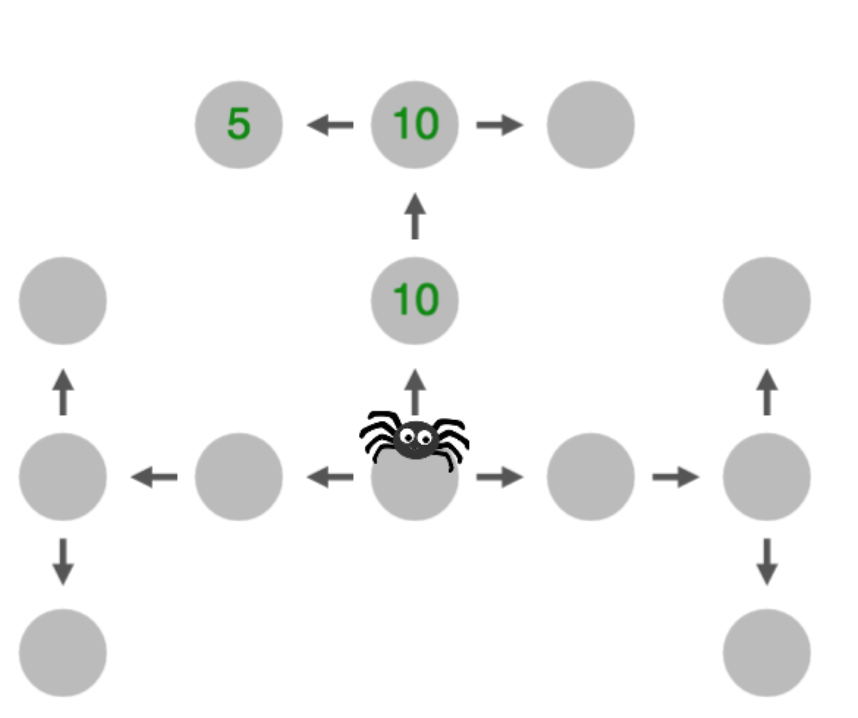
\includegraphics[width=0.4\textwidth]{figures/web-of-cash.png}
    \label{fig:MouselabMDP}
    \caption{Illustration of the Mouselab-MDP paradigm.}
\end{figure}


\section{Experiments}
\label{sec:experiments}

% For each experiment
%   Describe experiment-unique structure
%   Derive qualitative predictions
%   Results
%   Qualitative predictions
%   Quantitative model comparisons

% Experiment 1: effect of increasing vs. decreasing variance
% Experiment 2: effect of low vs. high variance
% Experiment 3: branching and depth


\section{Conclusion}
\label{sec:conclusion}

\paragraph{Summary and Interpretation of the results}
\fl{TODO: Fred, Priyam, Falk, Paul, and Sayan}

\paragraph{Implications and future directions}
\fl{TODO: Falk and Fred}

\bibliographystyle{apacite}

\setlength{\bibleftmargin}{.125in}
\setlength{\bibindent}{-\bibleftmargin}

\bibliography{references}


\end{document}
